%# -*- coding: utf-8-unix -*-
%%==================================================
%% chapter01.tex for SJTU Master Thesis
%%==================================================

%\bibliographystyle{sjtu2}%[此处用于每章都生产参考文献]
\chapter{系统实现}
\label{chap:systemimpl}
本章在上一章的基础上,介绍DOBBS在实现过程中所用到技术以及各个模块的具体实现情况。

\section{系统模块实现}
\begin{figure}[!htp]
    \centering
    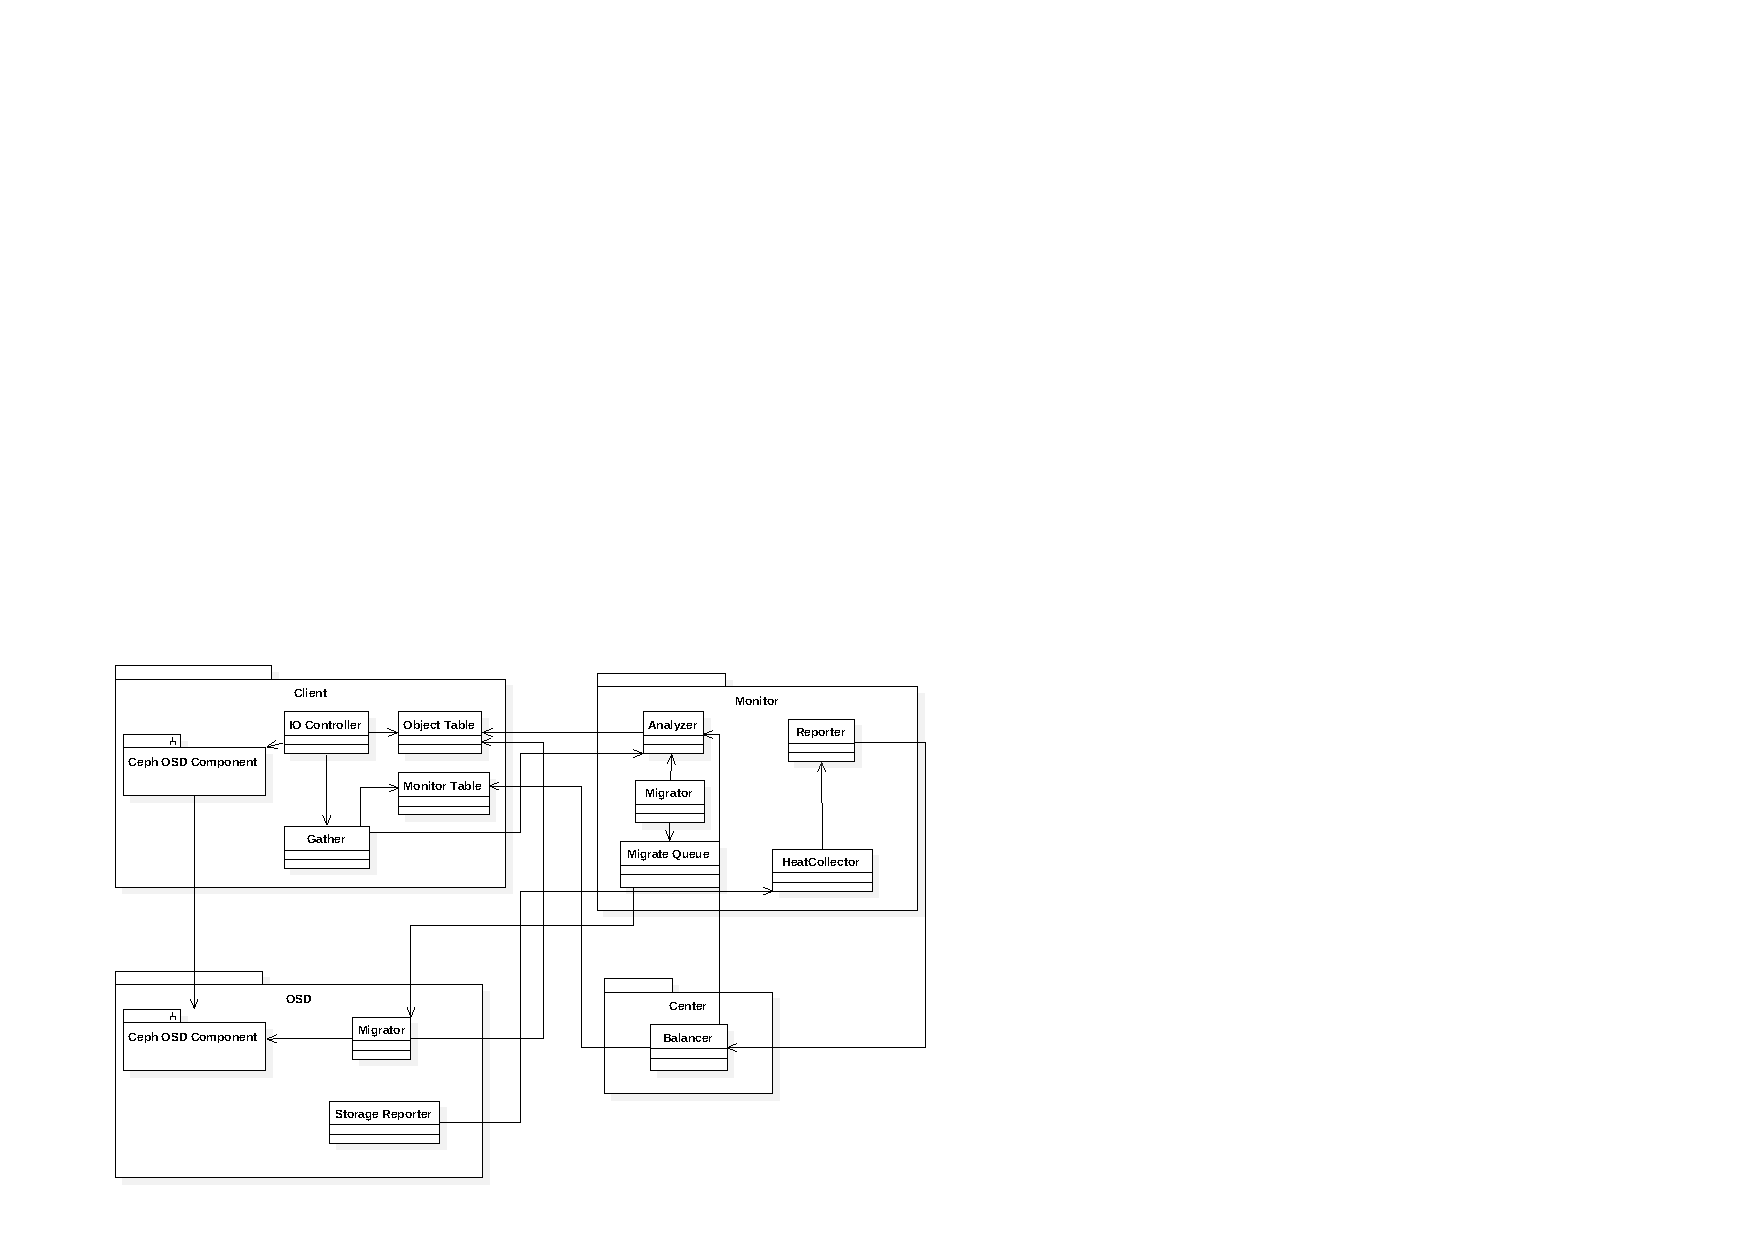
\includegraphics[width=15cm]{example/implmain.pdf}
    \bicaption[fig:implmain]{DOBBS模块结构}{DOBBS模块结构}{Fig}{Module Structure of DOBBS}
\end{figure}

如图\ref{fig:implmain}是系统模块结构图。从图中可以看到,DOBBS主要有四个组件,分别是客户端(Client)、监控器(Monitor)、OSD和中心控制器(Center)。
而我们的各个模块分布在了这些组件上。在本章系统实现部分我们不在用模块的概念来表述,图\ref{fig:implmain}的类则对应了上一张系统架构图中的各个模块。为了
直观显示DOBBS各个组件之间的关系,我们将Center独立出来作为一个组件描述,而实际场景中,Center是位于某个Monitor服务器上运行的。值得注意的是,图中的Ceph OSD Component
并不是DOBBS中的组件而是Ceph系统所提供的访问数据对象的接口。

Client主要包含四个类,这四个类也是与系统设计中的模块一一对应的。IO Controller用来截取VM的数据请求,并通过查询Object Table的方式来获取对象所在的OSD编号,再把对象ID和所在OSD编号共同
传递给Ceph OSD Component进行数据访问。IO Controller还有就是需要调用Gather的接口来记录VM访问对象的访问类型和ID。Object Table的主要作用是保存一个对象ID到OSD ID映射的数据结构,并暴露出
可以让IO Controller进行查询的接口,另外在局部热均衡对象迁移结束之后OSD上的Migrator也需要调用Object Table提供的更新映射的接口。Gather则用于收集对象的访问信息,并调用Monitor上的接口将
单位时间的数据流信息汇报给Monitor的Analyzer。而Monitor Table是用于存储Monitor ID与OSD ID的数据结构,因为全局热均衡会改变系统的逻辑结构,所以在全局热均衡结束之后会去更新Monitor Table提供的更新映射的接口。Gather则用于收集对象的访问信息,并调用Monitor上的接口将
值得注意的是,Gather在汇报给Monitor的时候需要先通过对象的OSD查询到该OSD在哪个子集群,然后在将相同子集群的对象数据流信息整合起来打包发送给对象的Monitor。

Monitor则包含五个类。Analyzer是用于接收Client的Gather所汇报的数据流信息,并且它内部会持续计算对象热度,在生成对象迁移策略之后调用Migrator发送迁移请求,Analyzer的另一个重要功能就是接受Center节点的命令开始热扩散的使能过程。
Migrator则主要负责对象的迁移请求发送等。Migrator Queue的主体是一个队列,用于存储迁移请求,另外Migrator Queue还会额外记录子集群当前迁移数量。Heat Collector是在全局热均衡中所用的类,它的主要作用是调用操作系统
指令获得Monitor的CPU和内存利用率,还有就是调用所在子集群OSD上的Storage Reporter接口获取存储设备的IOPS。Reorter则是会调取HeatCollector提供的接口获得实时子集群热度值,并定时将这个值
发送给Center的Balance。Center上的Balancer的主要功能就是接受Monitor发送的子集群热度值,然后运行算法\ref{algo:imbadect}生成热扩散请求,在热扩散结束之后再修改所有Client上的Monitor Table。


\subsection{Monitor的模块实现}
\begin{figure}[!htp]
    \centering
    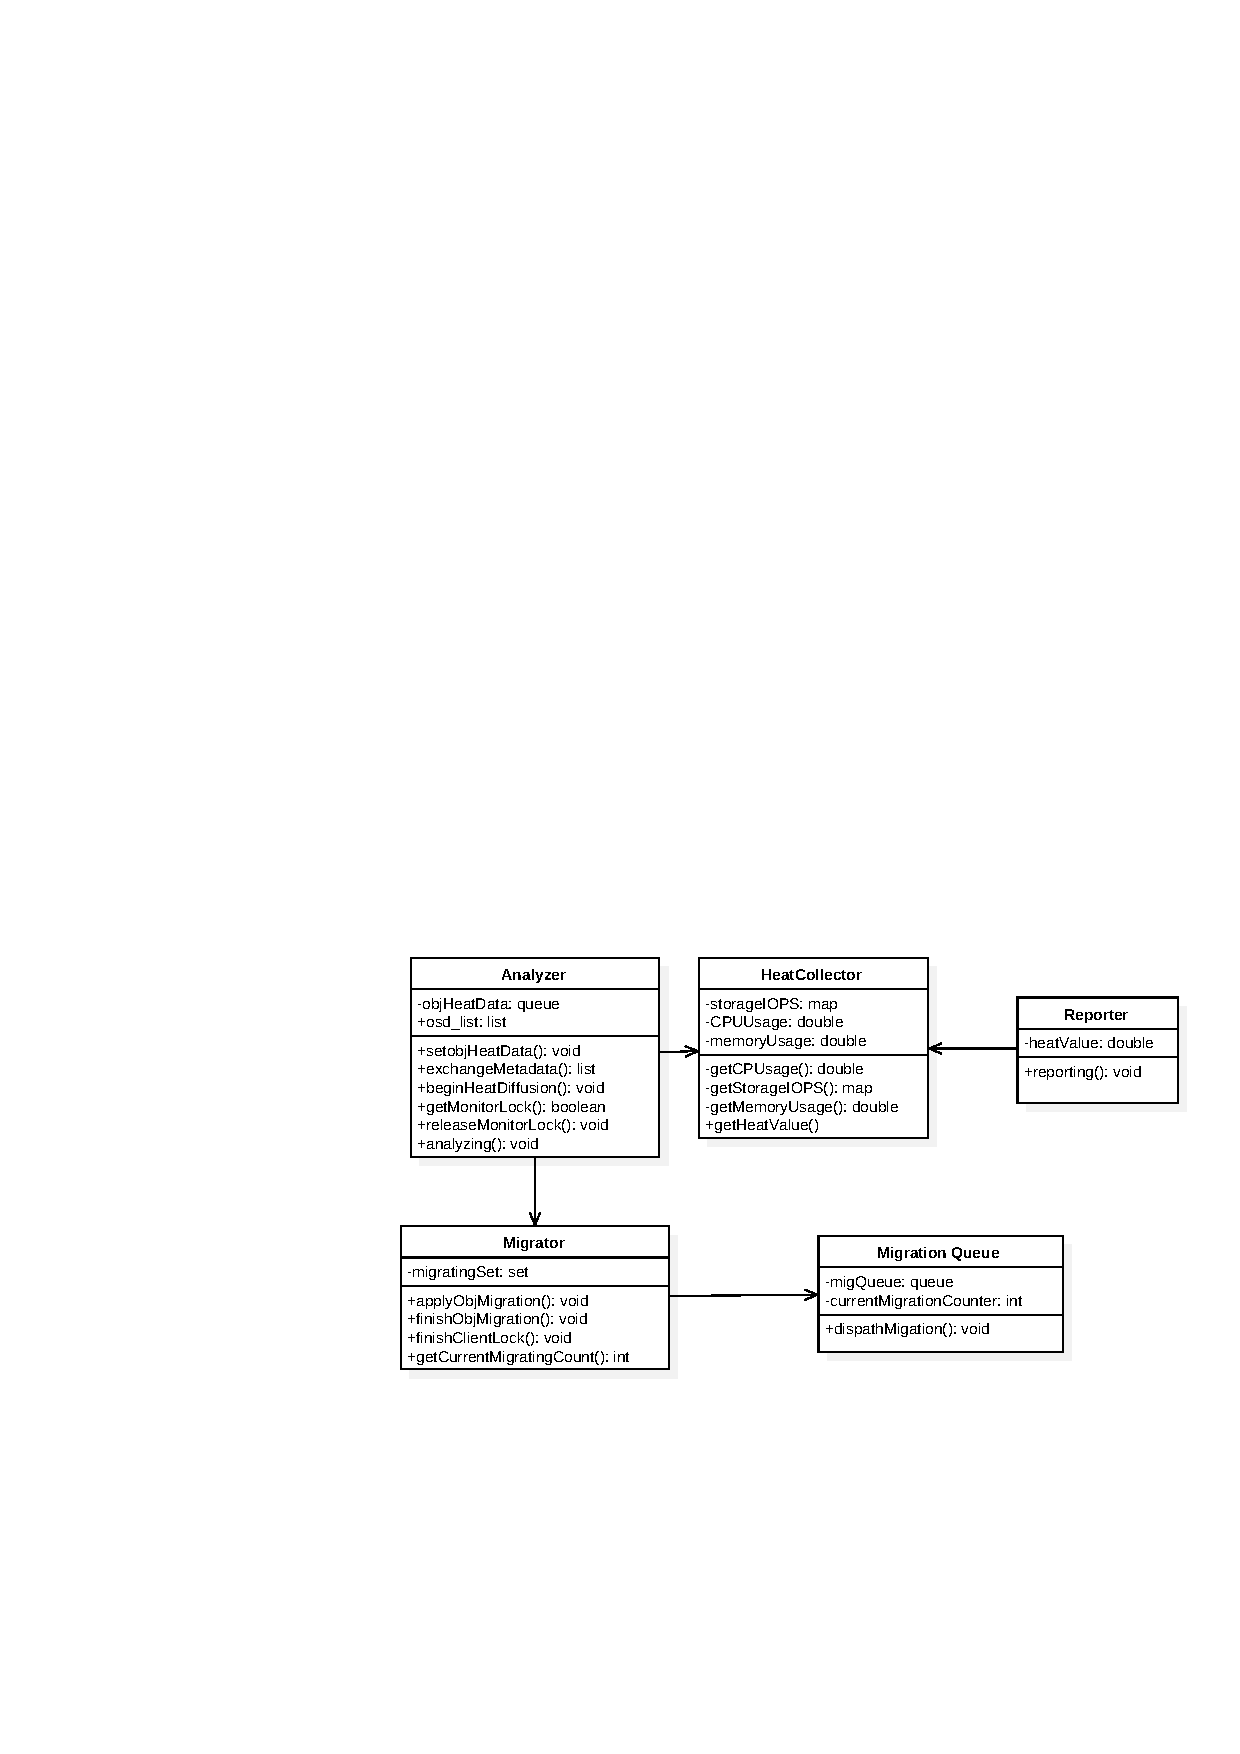
\includegraphics[width=12cm]{example/implmon.pdf}
    \bicaption[fig:implmon]{监视器模块类图}{监视器模块类图}{Fig}{Class Diagram of Monitor}
\end{figure}

图\ref{fig:implmon}所示是Monitor模块的设计类图。从图中可以看到Monitor一共有五个主要的类,其中的Analyzer、Migrator和Migrator Queue是继承于WHOBBS的实现\cite{lingxuan2015whobbs}。在本小结中,我们只做
简单的介绍,但是我们扩展了原有Analyzer类的功能,如全局热均衡的使能过程。

\subsubsection{Analyzer}
Analyzer的主要功能就是在局部热均衡的时候保存数据对象的热度信息,然后不断分析所有数据对象,计算对象的热度,并产生对象迁移请求。objHeatData是一个有序队列,我们实现了一个叫做ObjectQueue<typename T>的内置类,它内部是通过链表事先的
队列结构,只不过在链表插入的时候是根据元素的热度值进行的降序排序,保证了对头的元素的热度值总是最大的。objHeatData实际上的类型是ObjectQueue<ObjInfo>,ObjInfo是我们用来表示对象热度信息的结构体,这个结构体包含对象ID(oid)、所在
OSD编号(osd\_id)、所属Client IP(Client IP)和热度(heat\_val)。因此objHeatData是用于存储对象热度信息的,它通过heat\_val降序排序。Analyzer还有个数据结构是osd\_list,他的类型是std::list<int>,它用来存储当前子集群所包含的OSD
编号。

analyzing()方法是一个线程入口函数,Analyzer在被实例化之后就会启动分析线程。分析线程工作就是不断遍历objHeatData,产生对象迁移请求。根据上一章对Monitor的设计,analyzing遍历时候的策略就是将会维护一个当前SSD剩余容量的计数,在SSD的容量
没有满的时候,它会把objHeatData的前若干个对象放置于SSD上。那么如果一点SSD的容量已满,则会遍历objHeatData的前N个对象,N的大小等于SSD容量/单个对象大小,如果这前N个对象在SSD上,则不做迁移,反之则将其迁入HDD\cite{lingxuan2015whobbs}。
该分析线程发送迁移指令是通过调用Migrator的applyObjMiration()的接口来实现的。setObjData()接口的实现相对简单,它只是用来在Monitor接收到Client汇报来的数据流对象,通过热度计算算法计算出每个对象的热度之后,如果objHeatData中含有这个对象
则更新它的热度值,否则实例化一个ObjInfo对象,将它插入objHeaData中。

beginHeatDiffusion()、getMonitorLock()、releaseMonitorLock()和exchangeMetadata()这两个接口是Center所调用的。getMonitorLock()是用于对局部热均衡上锁,他会先去调用Migrator的getCurrentMigratingCount()接口获取现在子集群是否还有正在迁移的对象,如果接口返回值非0,则
不能上锁,接口返回false。如果getCurrentMigratingCount()的返回值是0,则会对analyzing()上锁并返回true,上锁我们是通过Linux的互斥锁pthread\_mutex\_t来实现的。beginHeatDiffion()接口是Center检测到子集群热度不均衡之后,并对Monitor
上锁之后执行的接口。这个接口就是全局热均衡使能过程的开始。而releaseMonitorLock()接口是Center在全局热均衡使能过程之后用于释放Monitor锁的,它调用pthread\_mutex\_unlock()这个Linux线程函数来解除加载analyzing线程上的互斥锁。

beginHeatDiffusion()接口传入的参数是目的子集群Monitor的IP地址。在接口开始调用的时候,他会调用HeatCollector的getStorageIOPS()接口,这个接口会返回子集群的存储集群各个OSD的编号和IOPS的映射。在获得这个映射之后,它找到最大IOPS的OSD编号。
然后它会去objHeatData中去遍历,找到所有osd\_id为IOPS最大OSD的对象,将他们从队列中剔除并置于一个传输buffer中。在封装完成后,它通过thrift调用目标子集群Monitor的exchangeMetadata()接口以参数的方式将buffer中的元数据传输给目标子集群。目标子集群
会从接口exchangeMetadata()其最“冷”OSD所对应的元数据,返回值类型为std::list<ObjInfo>。beginHeatDiffusion()在接受到返回值之后,把列表中的数据插入其自身的objHeatData,在接口执行的最后它会更新osd\_list中值,最后她调用Center的finishDiffusion()
方法。exchangeMatadata()接口则是在目标子集群的Monitor上被调用的接口,它的参数是源子集群最“热”OSD对应的元数据。该接口被调用之后,它会通过查询HeatCollector,找到IOPS最低的OSD编号,并将它所对应的元数据从onjHeatData中剔除,并通过返回值的方式传送给源子集群。

\subsubsection{Migrator和Migrator Queue}
Migrator和Migrator Queue的实现与WHOBBS中的实现相似,我们这里不再详细叙述这两个模块的实现。Migrator主要向Analyzer提供applyObjMigration()接口,Analyzer调用该接口后,该接口的传入参数是一个表示对象迁移的数据接口,然后它会调用Client上的上锁接口,在上锁成功后将迁移请求放置于Migrate Queue。
finishObjMigrating()接口是在OSD结束对象传输之后调用的,调用之后会把这个对象从migratingSet中剔除,然后调用Client上的释放锁的接口\cite{lingxuan2015whobbs}。与WHOBBS不同的是,为了支持Monitor锁,我们增加了getCurrentMigratingCount()接口,这接口在调用之后会直接返回当前migratingSet的大小。
migratingSet是在发送请求之后将oid放入其中,直到迁移完成后才会把它从migratingSet删除掉,因此migratingSet表示的是当前正在迁移对象的ID。Migrator Queue的实现与WHOBBS无异,本在则不再叙述。

\subsubsection{HeatCollector}
HeatCollector的功能是获取子集群的所有事实资源信息的。它主要有三个成员变量,分别是storageIOPS(存储集群IOPS)、CPUUsage(Monitor的CPU利用率)和memoryUsage(Monitor的内存利用率)。其中storageIOPS的数据类型是std::map<int, long>,这个map数据结构的键为osd\_id,值为对应OSD的IOPS值。
CPUUsage和memoryUsage的类型都是double,即占用百分比。

collecting()是一个线程入口函数。在系统初始化之后,启动collecting线程,该线程的作用就是不断调用getStorageIOPS()、getCPUUsage()和getMemoryUsage()接口获得当前实时的子集群资源信息,并更新它的三个成员变量。对于getStorageIOPS()解救,它会从在Analyzer的osd\_list获取子集群所包含OSD的编号,
然后再调用本子集群的OSD上的getIOPS()接口,最后将最新的存储集群IOPS值以map的方式返回。getCPUUsage()接口则是调用Linux的系统调用查看/proc/stat文件来获取当前CPU利用率。getMemoryUsage()则调用sysinfo()系统调用来获得当前的内存利用率的。

\subsubsection{Reporter}
Reporter的功能则是汇总子集群的资源利用信息,并定时发送给Center。Reporter包含一个成员变量,就是当前子集群的实时热度是heatValue,它的类型是double。reporting()函数是一个线程入口函数,该线程的主要功能就是不断的调用HeatCollector的三个get接口,然后再使用公式\ref{eq:subheat}来计算
子集群当前的热度值,在每次获取之后都会调用Center的reportFromMonitor()接口把热度值传输给Center。

\subsection{Center模块实现}

\begin{figure}[!htp]
    \centering
    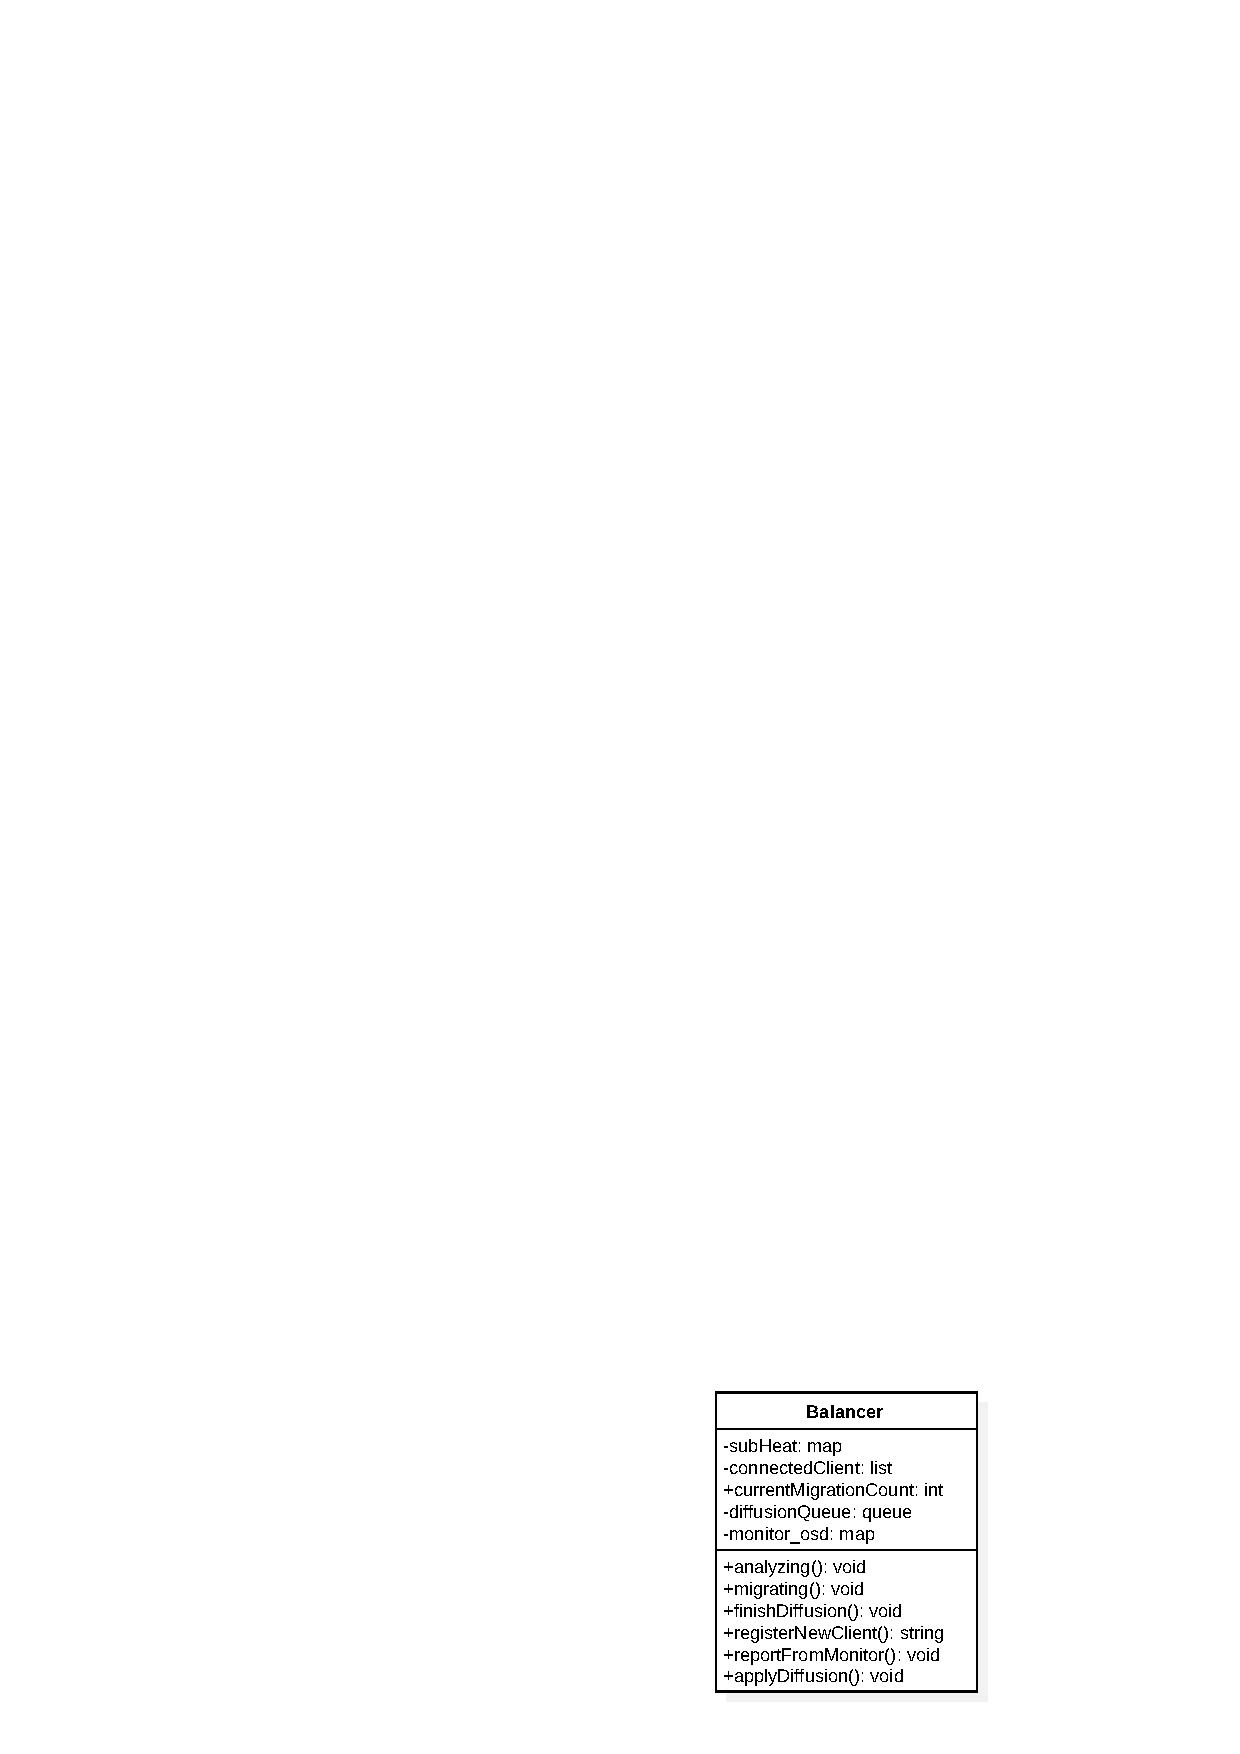
\includegraphics[width=5cm]{example/implcenter.pdf}
    \bicaption[fig:implcenter]{中心模块类图}{中心模块类图}{Fig}{Class Diagram of Center}
\end{figure}

如图\ref{fig:implcenter}所示为DOBBS的Center模块的类图,从图中可以看到Center只有一个叫做Balancer的类。Balancer类就实现了Center的所有功能,包括对各个子集群热度信息的收集、产生热迁移请求和新Client接入时的分配。

\subsubsection{Balancer}
Balancer主要有subHeat、connectedClient、currentDiffusionCount、diffusionQueue和monitor\_osd等五个成员变量。subHeat的数据类型的std::<std::string, double>,它表示各个子集群的热度值,其中的键为子集群id,值为热度值。connectedClient,它的类型是
std::list<std::string>表示当前接入系统的Client的IP地址。currentDiffusionCount表示当前正在全局热均衡的请求数量,它的类型是int。diffusionQueue表示准备进行热扩散的队列,它的类型是std::queue<DiffusionDetail>,DiffusionDetail是一个用来表示热扩散请求的结构体,
它包含to\_sub和from\_sub,即源子集群和目标子集群的编号。

Balancer的analyzing()函数是一个线程入口函数,这个线程主要就是用来运行子集群热度不均衡检测算法\ref{algo:imbadect},当算法找到源子集群和目的子集群之后会把原子群和目标子集群标号通过参数的方式传递给接口applyDiffusion()。而analyzing线程会过一定时间间隔
执行一次热度不均衡检测算法。reportFromMonitor()接口则是用于持续接受,各个Monitor所汇报的热度值信息。

applyDiffusion()算法在接收到源子集群编号和目标子集群编号之后,会生成一个DiffusionDetail类型的结构体,并将其放置于diffusionQueue中。migrating()函数则是迁移线程的入口函数,它的工作就是不断轮训diffusionQueue的内容,只要队列不为空它
会先检查currentDiffusionCount的值是否达到系统最大热扩散数量,如果已经达到则不对队列做任何处理。如果currentDiffusionCount小于系统最大热扩散数量,那么它会通过子集群编号调用两个子集群的getMonitorLock()接口,只有当两个都返回true时才将
这个热扩散请求从diffusionQueue删除。在这之后,它会调用源子集群的beginHeatDiffsion()接口,并将目标子集群标号传递给它。

finishDiffusion()结构是在源子集群和目标子集群结束全局热均衡的热值过程之后调用的,最终是有源子集群调用。在调用之后,Center会首先更新monitor\_osd的值,因为全局热均衡已经修改了子集群的逻辑结构。然后,Center再去更新通过connectedClient列表
去更新所有连接的Client的MonitorTable。最后则是调用目标子集群和源子集群的releaseMonitorLock()接口对两个Monitor解锁。

在上一章已经讲过,当Client初次接入系统时,Center会分配一个相对较“冷”的子集群给这个Client。在Client初次接入时,它会调用registerNewClient()接口,再把自己的IP地址通过传参的方式发送给Center。这个接口会遍历subHet,找到一个热度值最低的
子集群,然后将这个子集群Monitor的id返回给Client,最后Center把这个Client的IP置于connectedClient中。